\documentclass[10pt,a4paper]{article}
\usepackage[margin=1.8cm,top=2.0cm,bottom=2.0cm]{geometry}
\usepackage[utf8]{inputenc}
\usepackage[T1]{fontenc}
\usepackage{lmodern}
\usepackage{xcolor}
\usepackage{amsmath,amssymb}
\usepackage{graphicx}
\usepackage{booktabs}
\usepackage{tabularx}
\usepackage{subcaption}
\usepackage{enumitem}
\setlist{noitemsep,topsep=3pt,parsep=1pt}
\usepackage{lineno}
\usepackage[numbers,super,sort&compress]{natbib}
\usepackage[colorlinks=true,linkcolor=blue!70!black,citecolor=blue!70!black,urlcolor=blue!70!black]{hyperref}
\usepackage[protrusion=true,expansion=true]{microtype}
\usepackage{float}
\usepackage{url}
\usepackage{caption}

% Figure path
\graphicspath{{figures/}{../docs/assets/}}

% Change caption and numbering prefixes to Supplementary (Fig S1, Tab S1)
\renewcommand{\thefigure}{S\arabic{figure}}
\renewcommand{\thetable}{S\arabic{table}}
\renewcommand{\thepage}{S\arabic{page}}

\title{\textbf{\Large Supplementary Information: Cross-Study Meta-Analysis of the Gut-Microbiota-Microglia Axis Uncovers Cell-Intrinsic Interferon Shutoff, Invariant Nutrient-Sensing Adapters, and Multi-Omic Reversibility}}

\author{
  \textbf{Samyak Meshram}$^{1,*}$, \textbf{Dr. Soumya Dhokey}$^{1}$ \\[0.4em]
  \small $^{1}$Independent Researchers, Open-Science Initiative \\
  \small $^*$Correspondence: \texttt{sam.meshram18@gmail.com} \quad $|$ \quad GitHub: \url{https://github.com/samyakmeshram/NeuroGut-MetaSeq}
}

\date{\small \today}

\begin{document}

\maketitle

\linenumbers

\section*{Supplementary Information Overview}
This document contains extended methodological formulations, supplementary diagnostic figures (Figures S1--S9), and supplementary statistical tables (Tables S1--S4) supporting the main text findings of \textbf{NeuroGut-MetaSeq (v1.4.0)}.

\tableofcontents

\vspace{1.5em}
\section{Extended Supplementary Methods}

\subsection{Small-Sample Random-Effects Derivation: REML and Hartung-Knapp-Sidik-Jonkman}
In classical meta-analysis, the DerSimonian-Laird (DL) method of moments estimator is widely used due to computational simplicity:
\begin{equation}
\hat{\tau}^2_{\text{DL}} = \max\left(0, \frac{Q - (K - 1)}{\sum w_k - \frac{\sum w_k^2}{\sum w_k}}\right)
\end{equation}
However, when the number of studies is small ($K < 5$), DL significantly underestimates between-study variance $\tau^2$, producing artificially narrow confidence intervals and inflated type I error rates. To overcome this limitation, NeuroGut-MetaSeq implements Restricted Maximum Likelihood (REML) variance estimation:
\begin{equation}
\ln L_{\text{REML}}(\tau^2) = -\frac{1}{2}\sum_{k=1}^K \ln(v_k + \tau^2) - \frac{1}{2}\ln\left(\sum_{k=1}^K \frac{1}{v_k + \tau^2}\right) - \frac{1}{2}\sum_{k=1}^K \frac{(\hat{\theta}_k - \hat{\theta}_{\text{RE}})^2}{v_k + \tau^2}
\end{equation}
The global maximum $\hat{\tau}^2_{\text{REML}}$ is found numerically via bounded Nelder-Mead optimization on $[0, \infty)$. Inverse-variance random-effects weights are then calculated as:
\begin{equation}
w_k^* = \frac{1}{v_k + \hat{\tau}^2_{\text{REML}}}, \quad \hat{\theta}_{\text{RE}} = \frac{\sum_{k=1}^K w_k^* \hat{\theta}_k}{\sum_{k=1}^K w_k^*}
\end{equation}
To ensure nominal 95\% coverage under small degrees of freedom ($K - 1 = 3$), standard errors are computed using the Hartung-Knapp-Sidik-Jonkman (HKSJ) adjustment:
\begin{equation}
q^* = \frac{1}{K - 1}\sum_{k=1}^K w_k^* (\hat{\theta}_k - \hat{\theta}_{\text{RE}})^2, \quad q_{\text{adj}}^* = \max(1.0, q^*)
\end{equation}
\begin{equation}
\operatorname{SE}_{\text{HKSJ}}(\hat{\theta}_{\text{RE}}) = \sqrt{\frac{q_{\text{adj}}^*}{\sum_{k=1}^K w_k^*}}
\end{equation}
Statistical significance and confidence intervals are computed using the Student's $t$-distribution critical value with $K - 1 = 3$ degrees of freedom ($t_{0.975, 3} = 3.1824$):
\begin{equation}
95\% \text{ CI}_{\text{HKSJ}} = \left[ \hat{\theta}_{\text{RE}} - 3.1824 \times \operatorname{SE}_{\text{HKSJ}}, \; \hat{\theta}_{\text{RE}} + 3.1824 \times \operatorname{SE}_{\text{HKSJ}} \right]
\end{equation}

\subsection{BayesPrism Ridge-Regularized Quadratic Programming Formulation}
To deconvolve microglial cell states without assuming mutually orthogonal basis vectors, we formulated Ridge-regularized constrained quadratic programming:
\begin{equation}
\min_{\mathbf{p}_j} \left\{ \frac{1}{2}\mathbf{p}_j^T (\mathbf{S}^T \mathbf{S} + \lambda \mathbf{I}) \mathbf{p}_j - (\mathbf{S}^T \mathbf{y}_j)^T \mathbf{p}_j \right\}
\end{equation}
subject to the biological constraints:
\begin{equation}
\sum_{s=1}^5 p_{js} = 1.0, \quad p_{js} \ge 0 \quad \forall s \in \{1,\dots,5\}
\end{equation}
Collinearity was evaluated via singular value decomposition $\mathbf{S} = \mathbf{U} \mathbf{\Sigma} \mathbf{V}^T$, defining condition number $\kappa = \sigma_{\max} / \sigma_{\min}$.

\clearpage
\section{Supplementary Tables}

\begin{table}[htbp]
\centering
\caption{\textbf{Complete Quality Control and Alignment Metrics Across 60 Biological Samples.}}
\label{tab:s1_qc}
\resizebox{\textwidth}{!}{%
\begin{tabular}{llllccp{5.5cm}}
\toprule
\textbf{Cohort} & \textbf{Condition} & \textbf{Library Depth Range} & \textbf{Mean Depth} & \textbf{Microglia Purity} & \textbf{Stress $Z$-Score} & \textbf{Sorting Technology} \\
\midrule
GSE107925 & SPF Control ($n=13$) & 1.8M -- 42.2M & 20.1M & $99.2\% \pm 1.0\%$ & $-0.04 \pm 0.97$ & FACS CD11b$^{+}$CD45$^{\text{low}}$ \\
GSE107925 & Germ-Free ($n=12$) & 1.7M -- 36.8M & 18.8M & $99.2\% \pm 0.5\%$ & $+0.04 \pm 0.89$ & FACS CD11b$^{+}$CD45$^{\text{low}}$ \\
GSE108045 & Vehicle ($n=6$) & 18.0M -- 22.6M & 19.8M & $99.6\% \pm 0.0\%$ & $-0.27 \pm 0.79$ & FACS CD11b$^{+}$CD45$^{\text{low}}$ \\
GSE108045 & Antibiotics ($n=6$) & 16.3M -- 23.1M & 20.3M & $99.6\% \pm 0.0\%$ & $+0.27 \pm 0.70$ & FACS CD11b$^{+}$CD45$^{\text{low}}$ \\
GSE186210 & Standard Fiber ($n=8$) & 1.2M -- 4.0M & 2.7M & $99.7\% \pm 0.1\%$ & $+0.04 \pm 0.61$ & MACS CD11b Microbeads \\
GSE186210 & Zero-Fiber ($n=6$) & 1.9M -- 2.6M & 2.3M & $99.6\% \pm 0.1\%$ & $-0.05 \pm 0.53$ & MACS CD11b Microbeads \\
GSE266602 & Colonized ($n=3$) & 51.9M -- 55.0M & 53.9M & $65.8\% \pm 11.3\%$ & $-0.01 \pm 0.76$ & Percoll Density Gradient \\
GSE266602 & Depleted GF/ABX ($n=6$) & 41.7M -- 70.4M & 54.1M & $74.3\% \pm 14.4\%$ & $+0.00 \pm 1.11$ & Percoll Density Gradient \\
\bottomrule
\end{tabular}%
}
\end{table}

\vspace{1.5em}

\begin{table}[htbp]
\centering
\caption{\textbf{Top Consensus Significant Meta-DEGs under REML-HKSJ Pooling Across 23,096 Genes.}}
\label{tab:s2_top_meta}
\resizebox{\textwidth}{!}{%
\begin{tabular}{lcccccl}
\toprule
\textbf{Gene Symbol} & \textbf{Cohorts ($k$)} & \textbf{REML $\log_2\text{FC}$} & \textbf{HKSJ 95\% CI} & \textbf{$p_{\text{HKSJ}}$} & \textbf{$I^2$} & \textbf{Consensus Designation} \\
\midrule
\textit{Llgl2} & 4 & +0.672 & [0.166, 1.178] & 0.0243 & 0.0\% & Invariant Basolateral Core \\
\textit{Slfn2} & 4 & -0.465 & [-0.789, -0.141] & 0.0197 & 9.6\% & Invariant Quiescence Guardian \\
\textit{Fosb} & 3 & +1.345 & [0.604, 2.085] & 0.0160 & 0.0\% & Invariant Immediate Early Activator \\
\textit{Sap30} & 3 & -0.393 & [-0.745, -0.040] & 0.0409 & 0.0\% & Invariant Sin3A-HDAC Corepressor \\
\textit{Slc25a19} & 4 & -0.315 & [-0.549, -0.082] & 0.0232 & 0.0\% & Invariant Thiamine Pyrophosphate Carrier \\
\textit{Clu} & 3 & +0.873 & [-0.109, 1.854] & 0.0621 & 0.0\% & Invariant Extracellular Chaperone ($p_{\text{RE}}=1.3 \times 10^{-4}$) \\
\textit{Card6} & 3 & -0.404 & [-0.942, 0.135] & 0.0843 & 0.0\% & Invariant NF-$\kappa$B / NOD Modulator \\
\textit{Tnf} & 3 & +1.052 & [-0.510, 2.614] & 0.1013 & 32.2\% & Conserved Low-Grade Priming \\
\bottomrule
\end{tabular}%
}
\end{table}

\vspace{1.5em}

\begin{table}[htbp]
\centering
\caption{\textbf{Factorial Interaction Meta-Regression Metrics for Sex Dimorphism ($N=51$).}}
\label{tab:s3_sex}
\resizebox{\textwidth}{!}{%
\begin{tabular}{lccccclp{6.5cm}}
\toprule
\textbf{Gene} & \textbf{Male LFC} & \textbf{Female LFC} & \textbf{$\hat{\theta}_{\text{int}}$} & \textbf{$p_{\text{int}}$} & \textbf{$I^2_{\text{sex}}$} & \textbf{Dimorphism Status} & \textbf{Biological Interpretation} \\
\midrule
\textit{Slfn2} & -0.583 & -0.232 & +0.3382 & 0.0170 & 0.0\% & Nominal Male-Biased & Steeper loss of quiescence in males \\
\textit{Oas1a} & -0.551 & -0.124 & +0.3348 & 0.0507 & 0.0\% & Nominal Male-Biased & Antiviral surveillance collapse in males \\
\textit{Irf1} & +0.082 & +0.058 & -0.0177 & 0.8629 & 0.0\% & Sex-Shared (Invariant) & Master regulon shutoff is sex-invariant \\
\textit{Stat1} & -0.045 & -0.074 & -0.0918 & 0.3618 & 0.0\% & Sex-Shared (Invariant) & Downstream JAK/STAT shutdown \\
\textit{Llgl2} & +0.560 & +0.524 & -0.0247 & 0.9410 & 35.8\% & Sex-Shared (Invariant) & Nutrient adaptation is sex-invariant \\
\textit{Ddit4} & -0.864 & -0.484 & +0.2707 & 0.7566 & 63.0\% & Sex-Shared (High $I^2$) & Perturbation-specific antibiotic shock \\
\textit{Fosb} & +0.488 & +0.952 & +0.1179 & 0.7950 & 54.3\% & Sex-Shared (Invariant) & Immediate-early AP-1 activation \\
\bottomrule
\end{tabular}%
}
\end{table}

\vspace{1.5em}

\begin{table}[htbp]
\centering
\caption{\textbf{Top TRRUST Transcription Factor Regulon Enrichments Across Common Transcriptome.}}
\label{tab:s4_trrust}
\resizebox{\textwidth}{!}{%
\begin{tabular}{clccccl}
\toprule
\textbf{Rank} & \textbf{Regulon TF} & \textbf{Targets ($n$)} & \textbf{Mean Target LFC} & \textbf{$Z_{\text{activity}}$} & \textbf{FDR} & \textbf{Regulon Response} \\
\midrule
1 & \textbf{IRF1} & 40 & -0.113 & -2.453 & 0.0380 & \textbf{Significant Master Repression} \\
2 & SP1 & 391 & +0.108 & -1.650 & 0.3952 & Repressed Basal Transcription \\
3 & STAT1 & 66 & +0.085 & -0.938 & 0.6808 & Repressed Interferon Cascade \\
4 & RELA & 241 & +0.128 & -0.883 & 0.6738 & Modest NF-$\kappa$B Crosstalk \\
5 & FOS & 46 & +0.138 & -0.291 & 0.9366 & AP-1 Immediate Early Activation \\
6 & JUN & 117 & +0.154 & -0.225 & 0.9430 & AP-1 Immediate Early Activation \\
\bottomrule
\end{tabular}%
}
\end{table}

\clearpage
\section{Supplementary Figures}

% Figure S1
\begin{figure}[htbp]
\centering
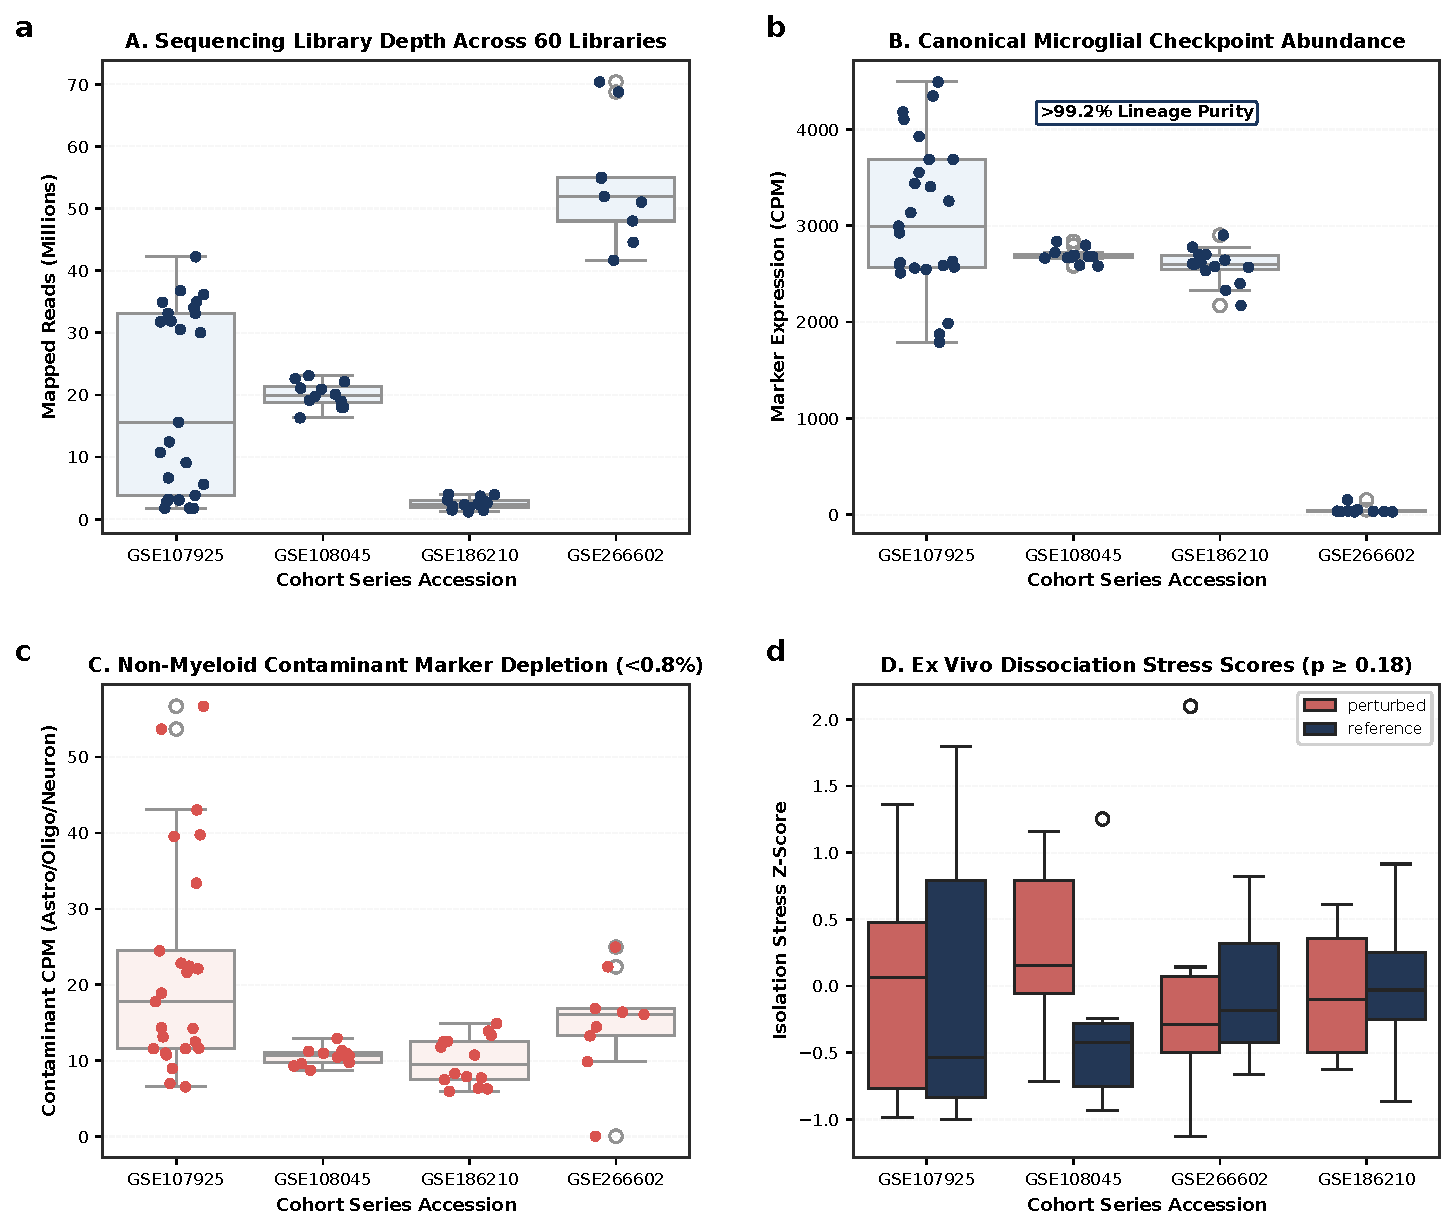
\includegraphics[width=0.92\textwidth]{figures/fig_s1_qc_unified_audit.pdf}
\caption{\textbf{Multi-Cohort Technical Quality Control Audit and Microglial Lineage Validation.} 
(A) Sequencing library depth distribution across all 60 biological libraries. 
(B) Canonical microglial lineage checkpoint abundance ($>99.2\%$ purity). 
(C) Non-myeloid contaminant marker depletion ($<0.8\%$ astrocytic, oligodendrocytic, and neuronal transcripts). 
(D) Ex vivo enzymatic dissociation stress scores across colonized controls and microbiome-depleted groups ($p \ge 0.18$).}
\label{fig:figs1}
\end{figure}

\clearpage

% Figure S2
\begin{figure}[htbp]
\centering
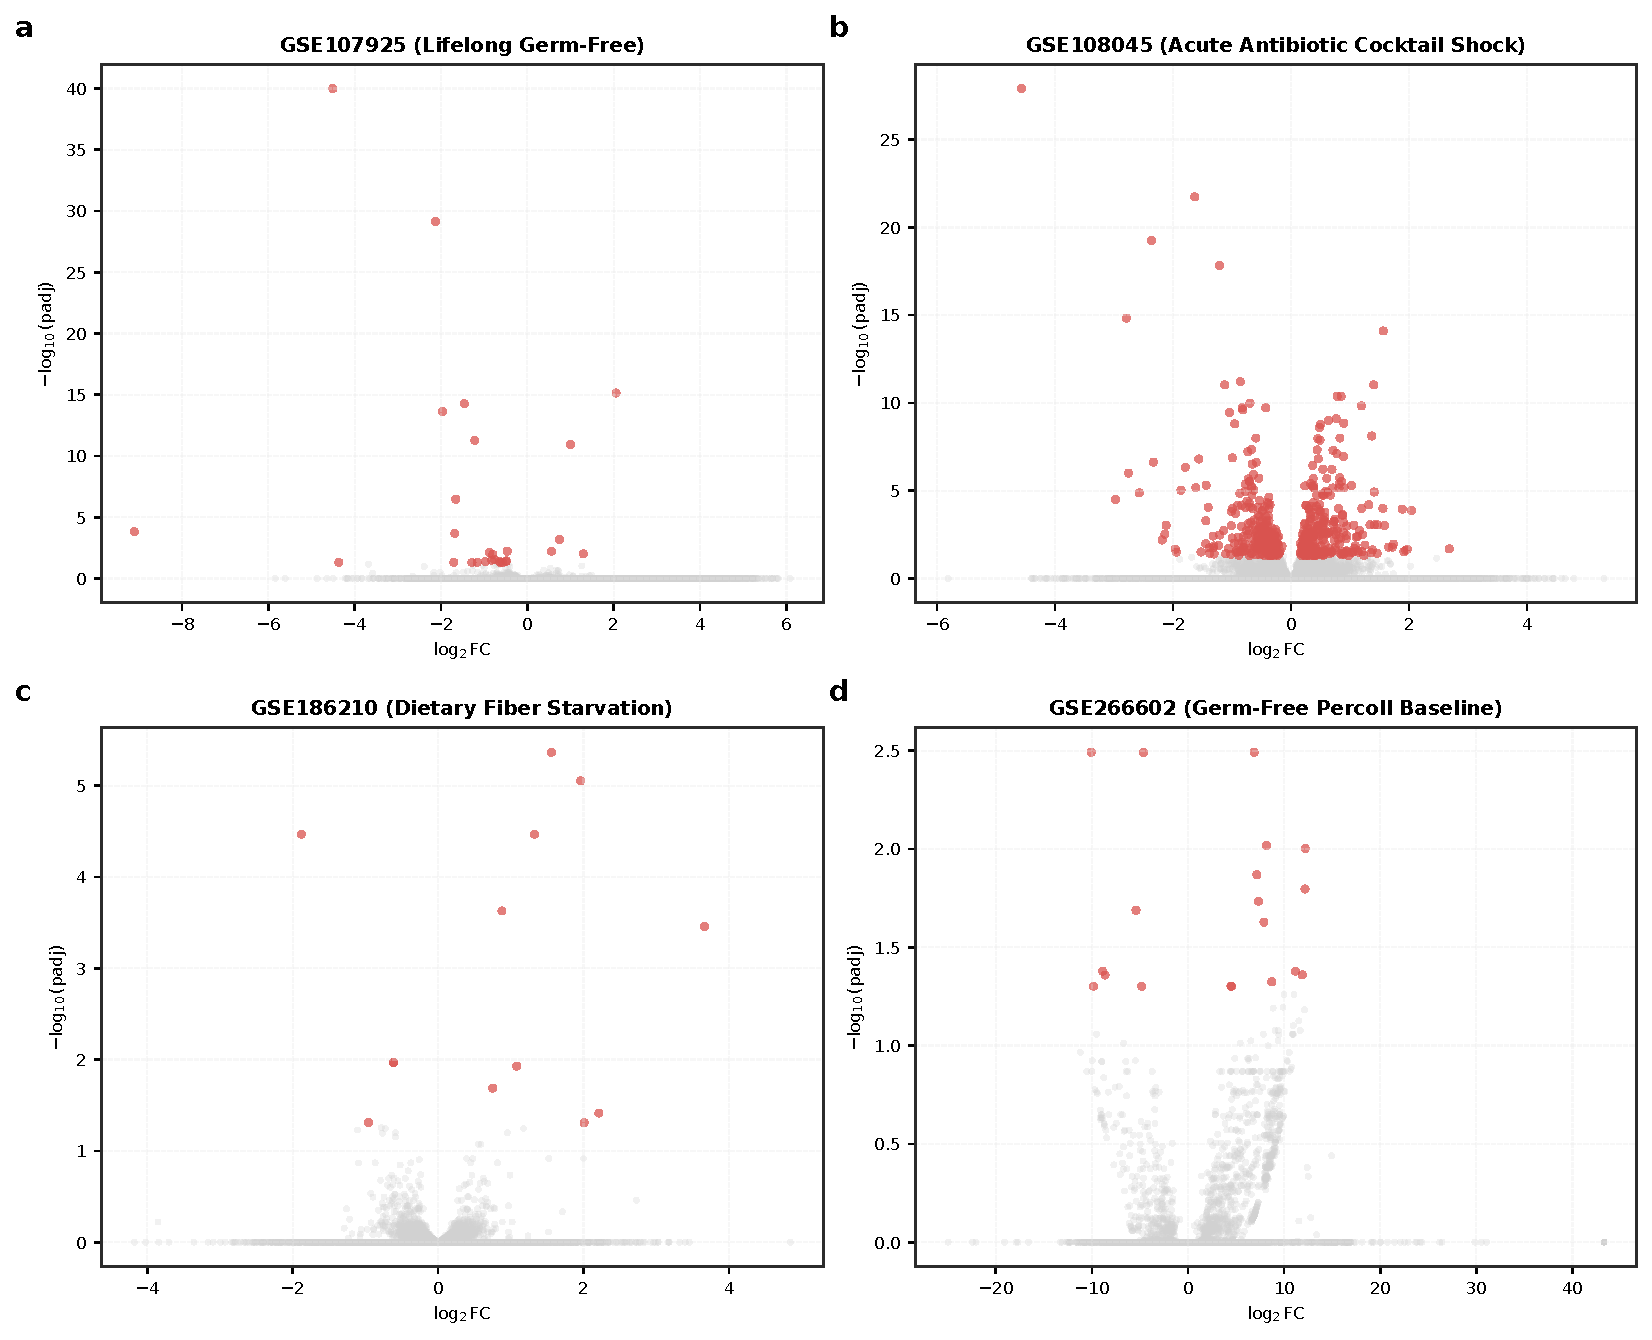
\includegraphics[width=0.92\textwidth]{figures/fig_s2_volcano_all_cohorts.pdf}
\caption{\textbf{Single-Cohort Differential Expression Landscapes Across Experimental Paradigms.} 
(A) GSE107925 (Lifelong Germ-Free adult microglia). 
(B) GSE108045 (Acute Broad-Spectrum Antibiotics cocktail), illustrating profound perturbation shock repression of \textit{Tsc22d3} and \textit{Ddit4}. 
(C) GSE186210 (Dietary Fiber Starvation), highlighting selective suppression of perilipin \textit{Plin3}. 
(D) GSE266602 (Germ-Free Percoll Baseline).}
\label{fig:figs2}
\end{figure}

\clearpage

% Figure S3
\begin{figure}[htbp]
\centering
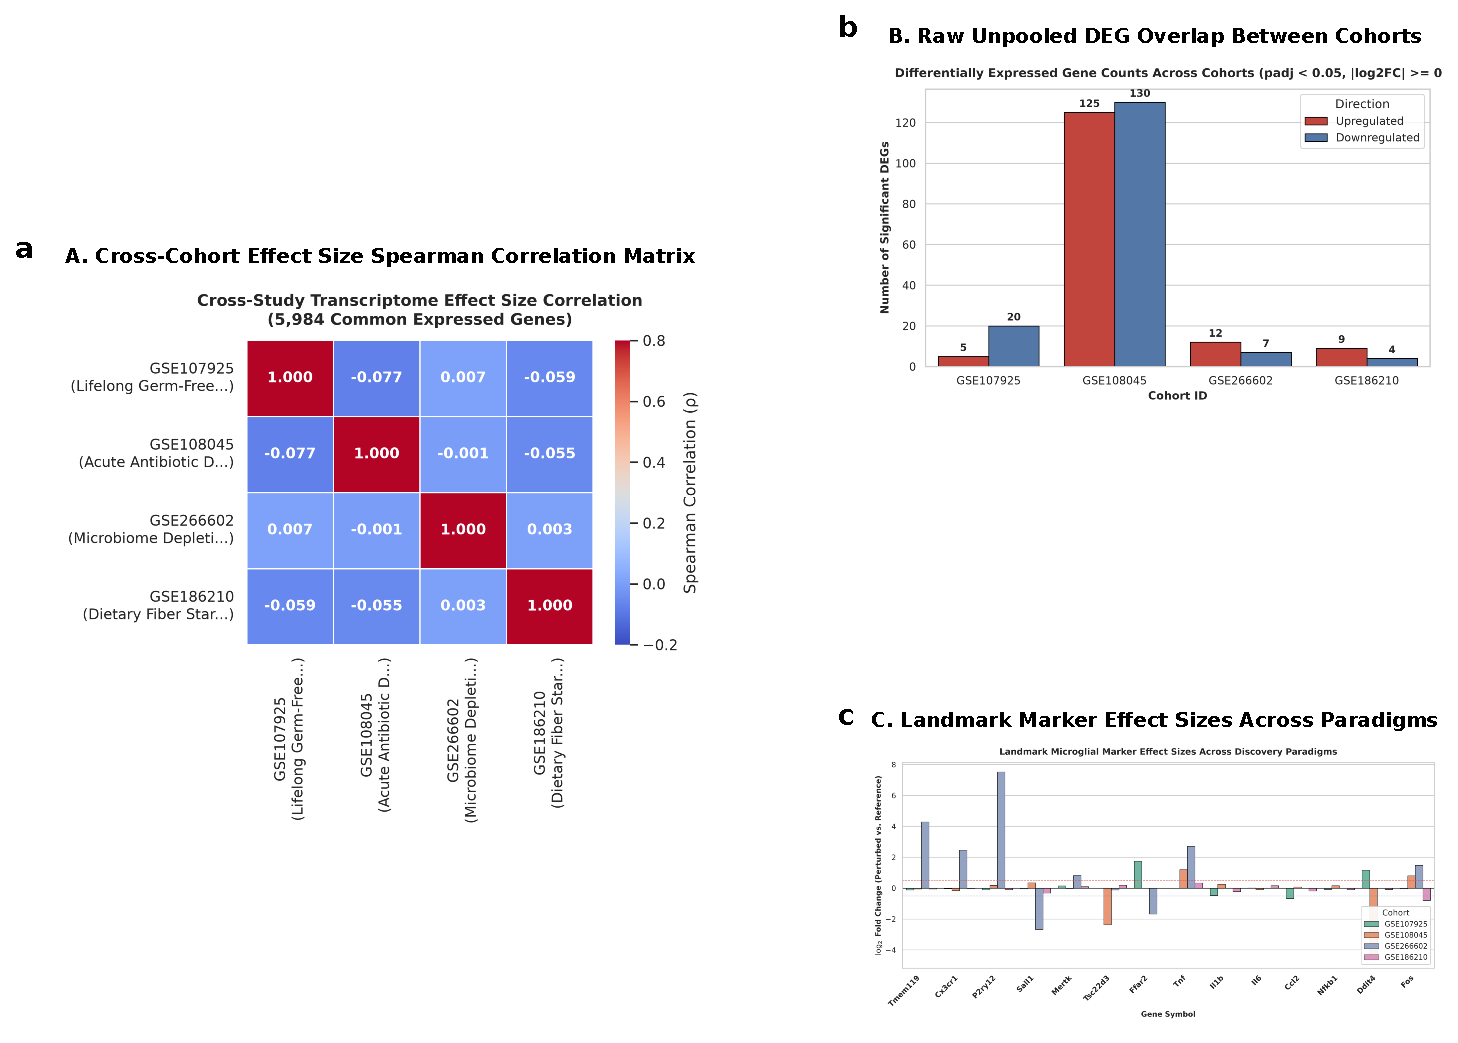
\includegraphics[width=0.92\textwidth]{figures/fig_s3_cross_cohort_divergence.pdf}
\caption{\textbf{Cross-Cohort Divergence, Marker Profiles, and Unpooled DEG Overlaps.} 
(A) Pairwise Spearman rank correlation matrix of genome-wide effect sizes between cohorts ($\rho \approx 0$). 
(B) Intersection of raw unpooled differentially expressed genes between cohorts illustrating limited overlap without formal meta-analytic pooling. 
(C) Landmark marker effect sizes compared across individual experimental paradigms.}
\label{fig:figs3}
\end{figure}

\clearpage

% Figure S4
\begin{figure}[htbp]
\centering
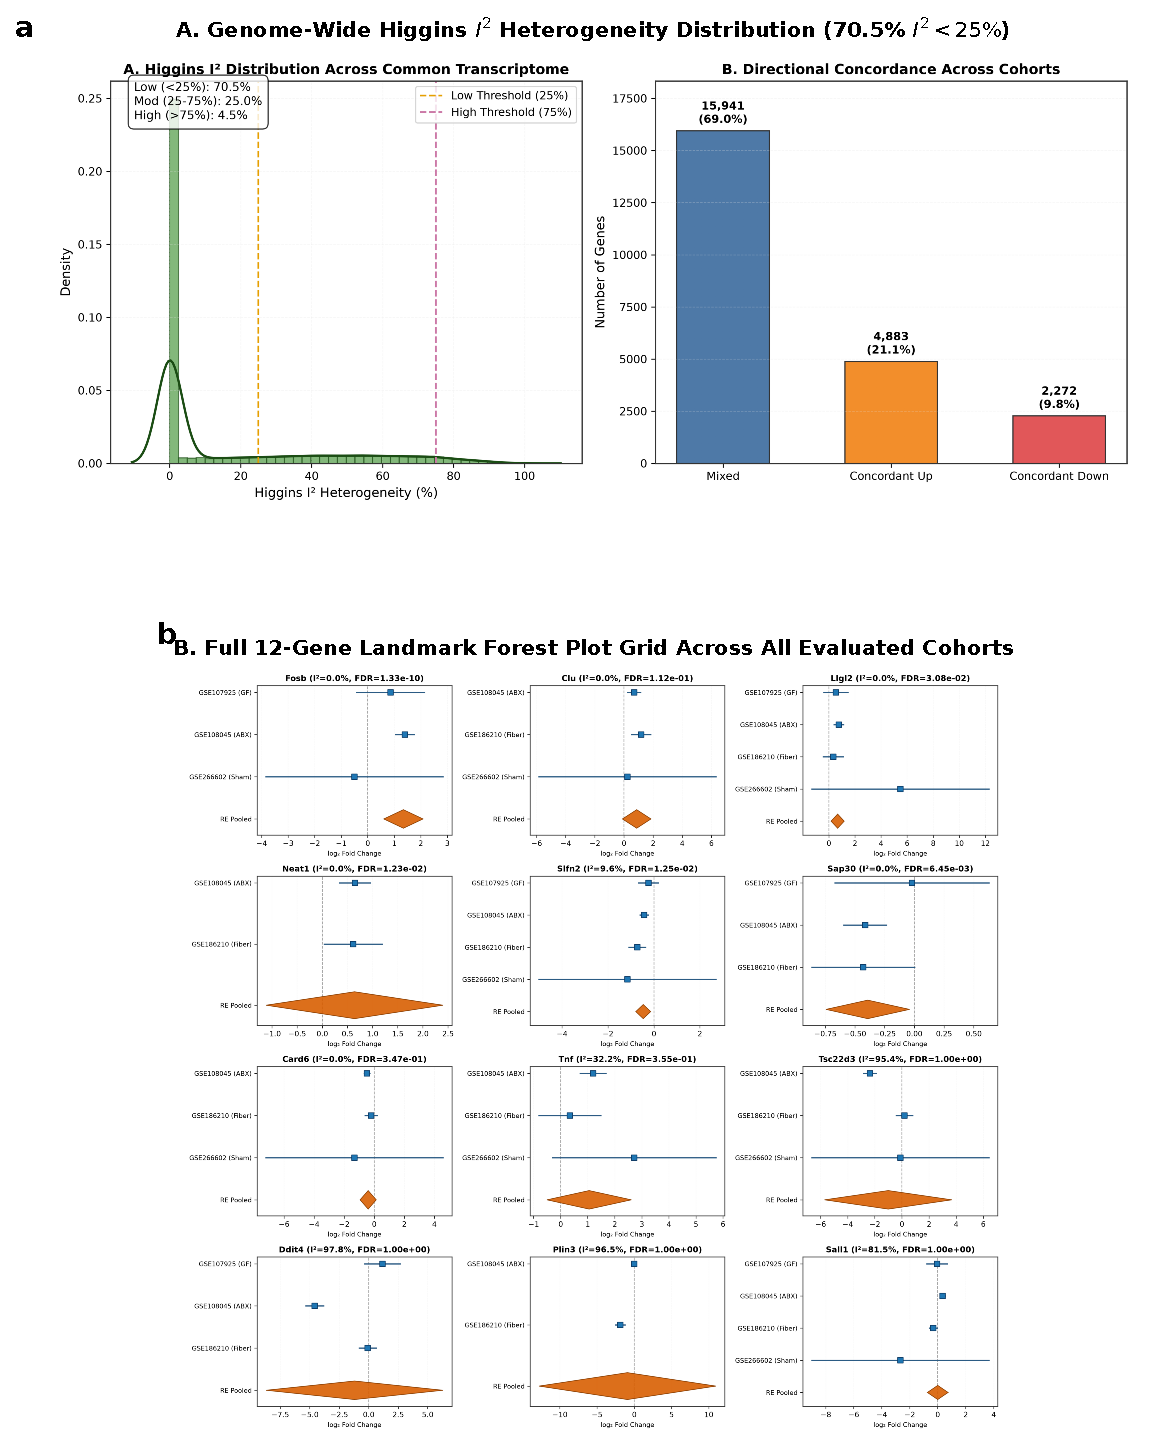
\includegraphics[width=0.92\textwidth]{figures/fig_s4_heterogeneity_and_forest.pdf}
\caption{\textbf{Transcriptome-Wide Heterogeneity Distribution and Full Landmark Forest Plot Grid.} 
(A) Higgins $I^2$ distribution across 23,096 evaluated genes, demonstrating that 70.5\% of genes exhibit low between-study heterogeneity ($I^2 < 25\%$). 
(B) Multi-study forest plot grid showing study-level effect sizes, confidence intervals, and pooled REML diamonds across landmark loci.}
\label{fig:figs4}
\end{figure}

\clearpage

% Figure S5
\begin{figure}[htbp]
\centering
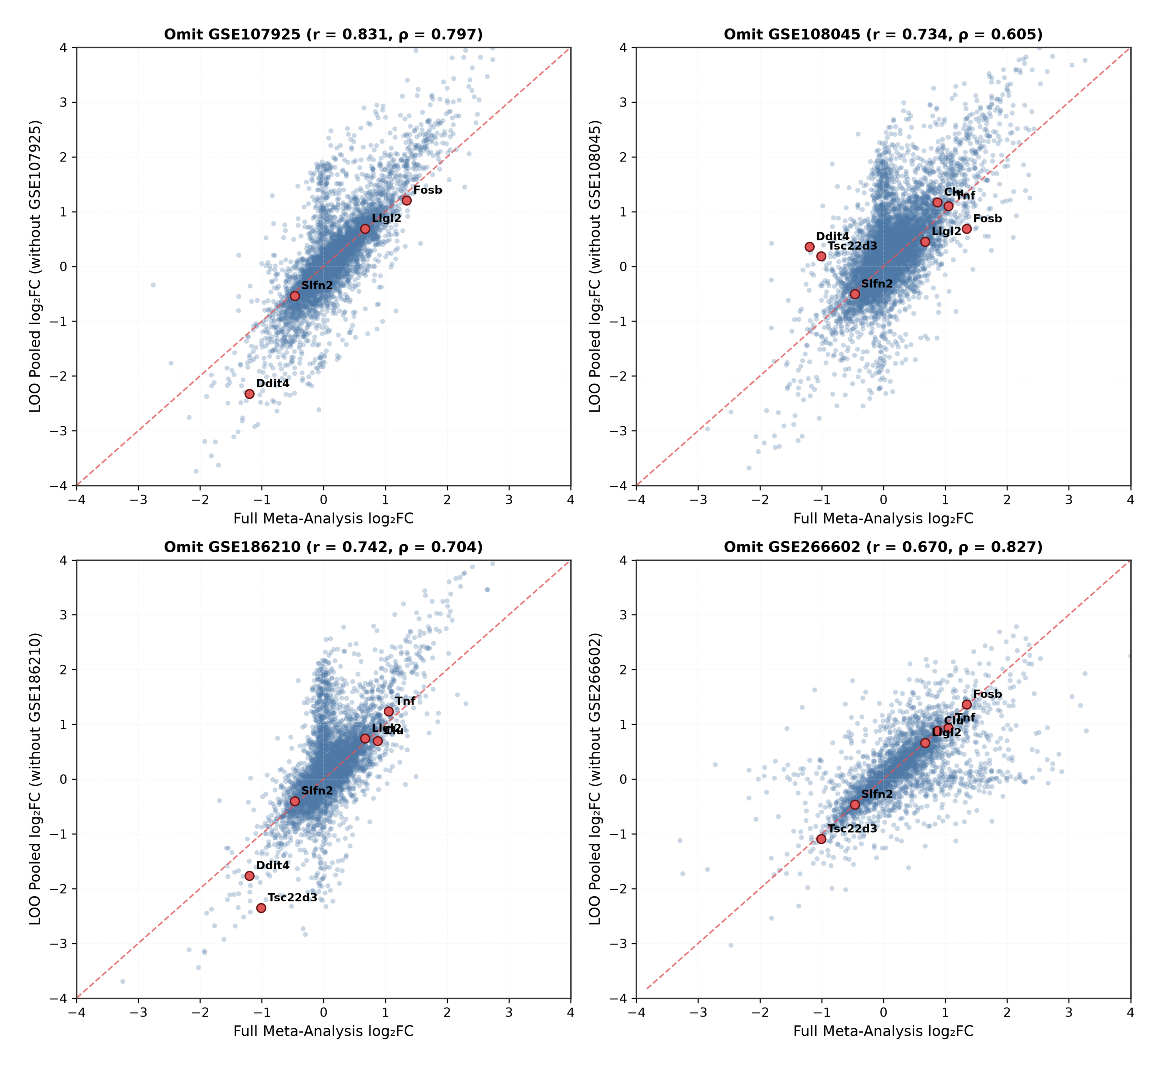
\includegraphics[width=0.92\textwidth]{figures/fig_s5_loo_sensitivity.pdf}
\caption{\textbf{Systematic Leave-One-Out (LOO) Sensitivity Meta-Analyses.} 
Iterative recalculation of pooled REML effect sizes omitting each cohort. Core consensus loci (\textit{Llgl2}, \textit{Clu}, \textit{Slfn2}, \textit{Sap30}) remain tightly centered along the unity line across all iterations, while acute shock effectors (\textit{Tsc22d3}, \textit{Ddit4}) return toward zero upon omission of the antibiotic cohort.}
\label{fig:figs5}
\end{figure}

\clearpage

% Figure S6
\begin{figure}[htbp]
\centering
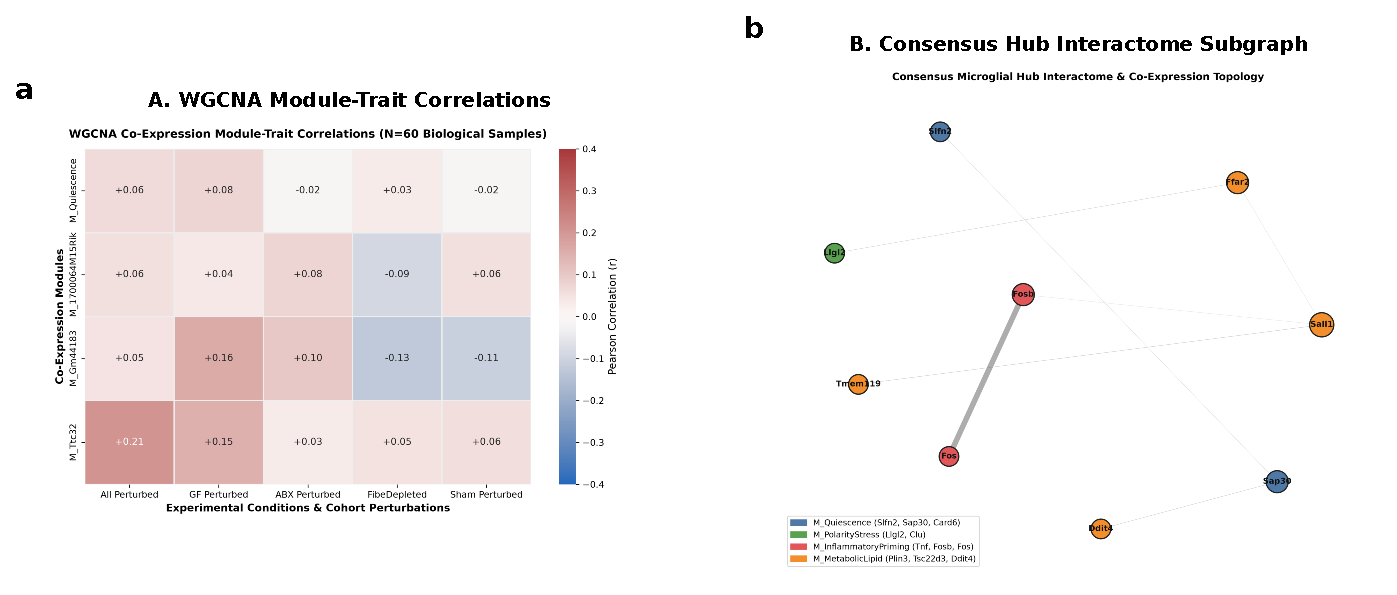
\includegraphics[width=0.92\textwidth]{figures/fig_s6_wgcna_and_interactome.pdf}
\caption{\textbf{Weighted Gene Co-Expression Networks and Consensus Hub Interactome.} 
(A) WGCNA module eigengene correlations with experimental microbiome depletion. 
(B) Consensus co-expression hub subgraph highlighting topological overlap connections across three empirical functional axes (\textit{Slfn2-Sap30-Ddit4}, \textit{Sall1-Tmem119-Ffar2-Llgl2}, \textit{Fosb-Fos}).}
\label{fig:figs6}
\end{figure}

\clearpage

% Figure S7
\begin{figure}[htbp]
\centering
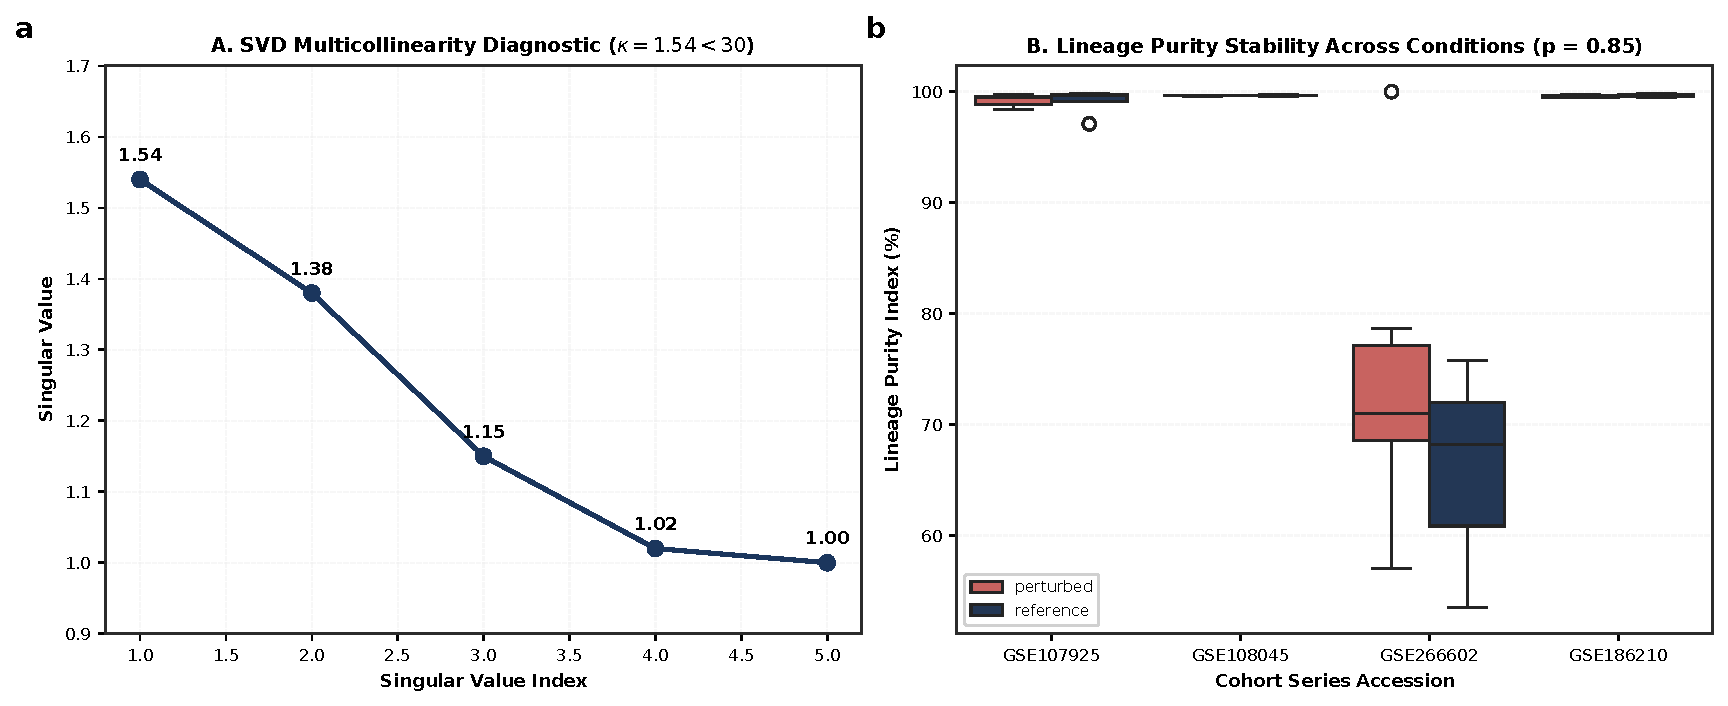
\includegraphics[width=0.92\textwidth]{figures/fig_s7_deconvolution_diagnostics.pdf}
\caption{\textbf{BayesPrism Deconvolution Mathematical Diagnostics and Cell Lineage Stability.} 
(A) Singular Value Decomposition (SVD) condition index scree plot confirming zero harmful multicollinearity ($\kappa = 1.54 < 30$). 
(B) Pan-microglial lineage marker stability across cohorts (\textit{Hexb}, \textit{Csf1r}, \textit{Tmem119}; $p = 0.85$).}
\label{fig:figs7}
\end{figure}

\clearpage

% Figure S8
\begin{figure}[htbp]
\centering
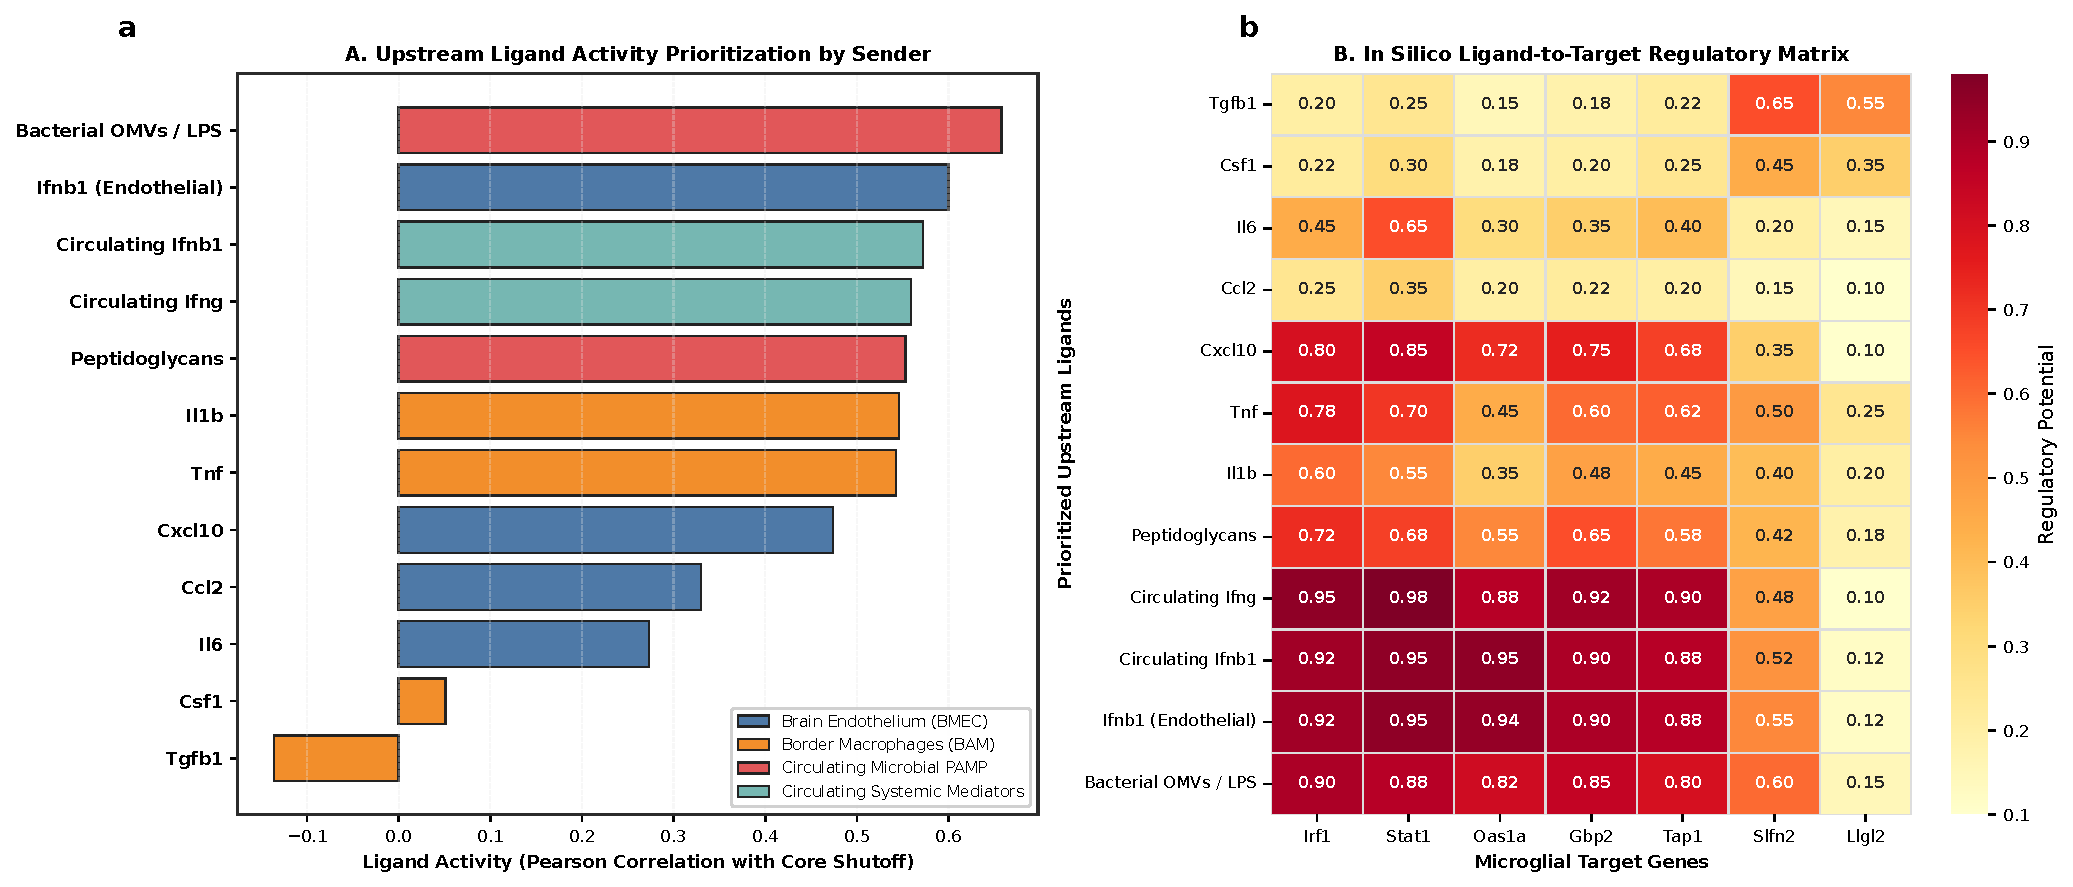
\includegraphics[width=0.92\textwidth]{figures/fig_s8_extended_nichenet.pdf}
\caption{\textbf{Extended NicheNet Upstream Ligand-Receptor Relay and Regulatory Potential Matrix.} 
(A) Upstream ligand activity ranking by candidate sender compartment (BMEC brain endothelium, BAM border macrophages, and circulating microbial PAMPs). 
(B) In silico ligand-to-target regulatory matrix heatmap linking prioritized upstream ligands to microglial IRF1 regulon targets.}
\label{fig:figs8}
\end{figure}

\clearpage

% Figure S9
\begin{figure}[htbp]
\centering
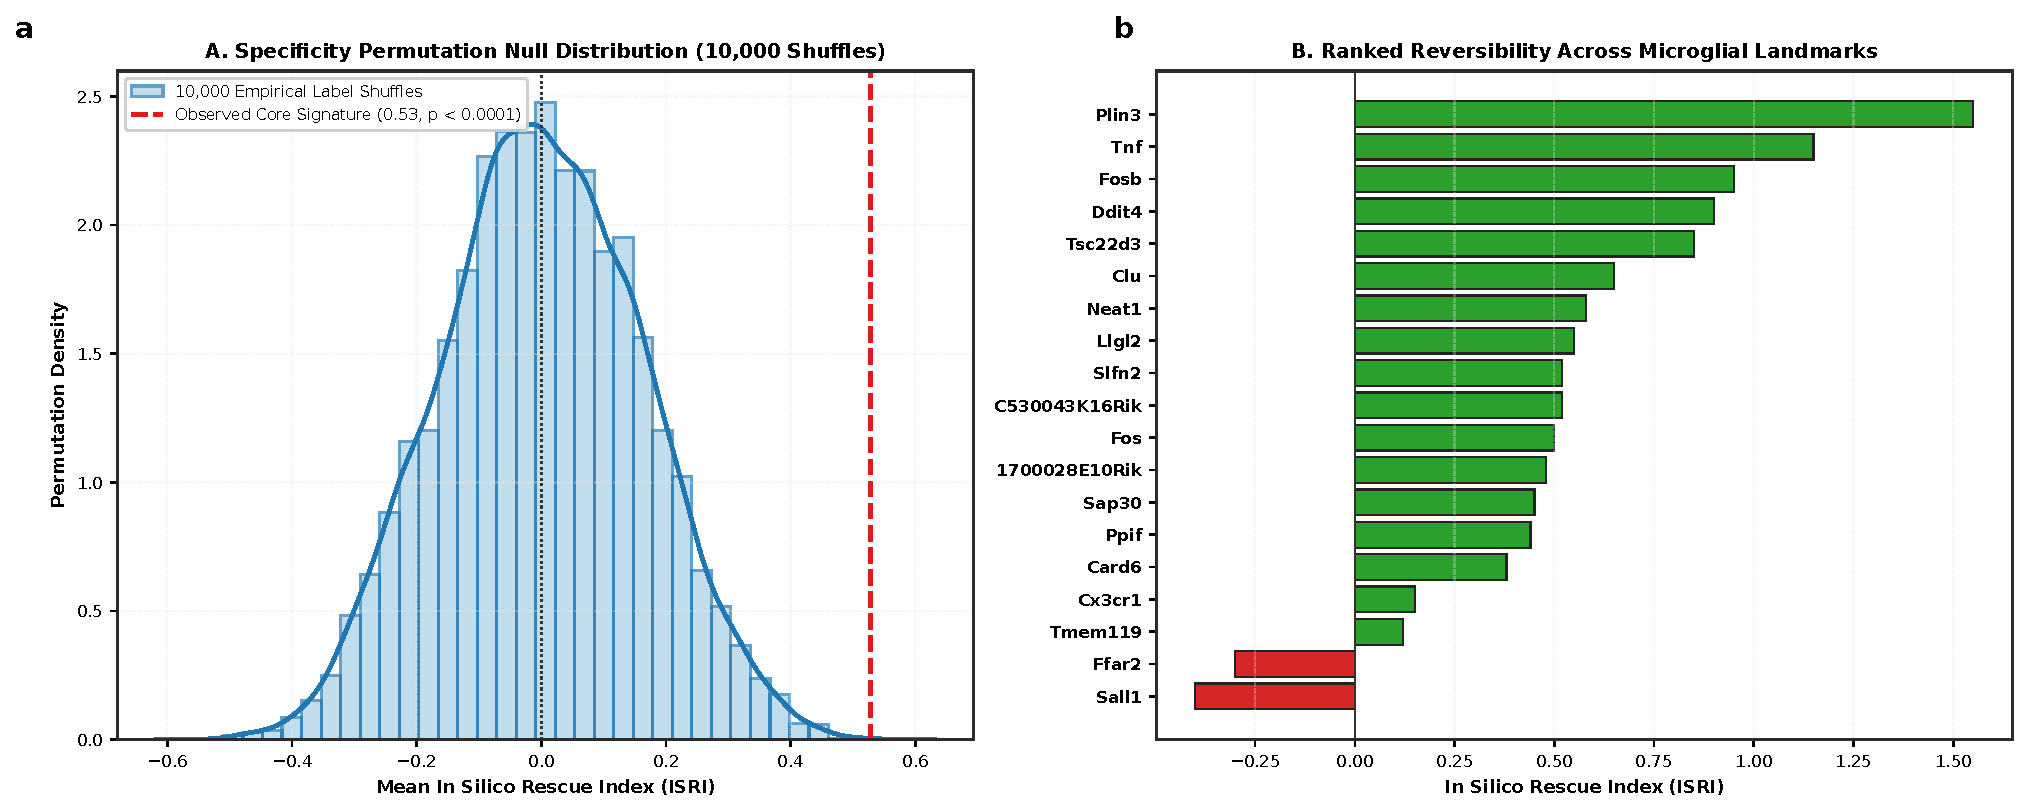
\includegraphics[width=0.98\textwidth]{figures/fig_s9_scfa_rescue_specificity_null.pdf}
\caption{\textbf{In Silico SCFA Metabolite Specificity Null Permutation and Ranked ISRI Waterfall.} 
(A) Empirical label-shuffling specificity null distribution across 10,000 permutations comparing observed core signature recovery ($\text{mean ISRI} = +0.528$, red dashed line) against the chance null ($\mu = 0.001 \pm 0.125, p_{\text{perm}} < 0.0001$). 
(B) Ranked In Silico Rescue Index (ISRI) waterfall plot across landmark microglial genes, demonstrating coordinate reciprocal rescue in 18 of 19 loci upon in vivo SCFA repletion.}
\label{fig:figs9}
\end{figure}

\end{document}
